%!TEX root = skripsi.tex
%-----------------------------------------------------------------------------%
\chapter{\babDua}
%-----------------------------------------------------------------------------%

%-----------------------------------------------------------------------------%
\section{Pengenalan Entitas Kesehatan}\label{aboutmer}
%-----------------------------------------------------------------------------%
% Apa itu MER
Pengenalan Entitas Kesehatan atau disebut juga dengan \textit{Medical Entity Recognition} (\mer) merupakan salah satu cabang dari Pengenalan Entitas Bernama (\textit{Named Entity Recoginition}) atau disingkat NER dengan dokumen sumber berupa teks kesehatan. NER sendiri merupakan suatu sistem/aplikasi yang memanfaatkan teknik pada \textit{Natural Language Processing} dan \textit{Information Extraction} untuk mengenali entitas yang telah dikategorikan sebelumnya seperti nama, lokasi, organisasi, waktu dan sebagainya. Sedangkan pada sistem MER, entitas yang akan dikenali yaitu entitas yang berada pada domain kesehatan seperti nama penyakit (\textit{\disease}), gejala penyakit (\textit{symptom}), obat (\textit{\drug}) dan langkah penyembuhan (\textit{\treatment}), nama protein, DNA, RNA dan lain sebagainya. Gambar \ref{fig:mer_ilustration} merupakan ilustrasi dari sebuah sistem \mer.

% Contoh tentang MER
\begin{figure}
	\centering
	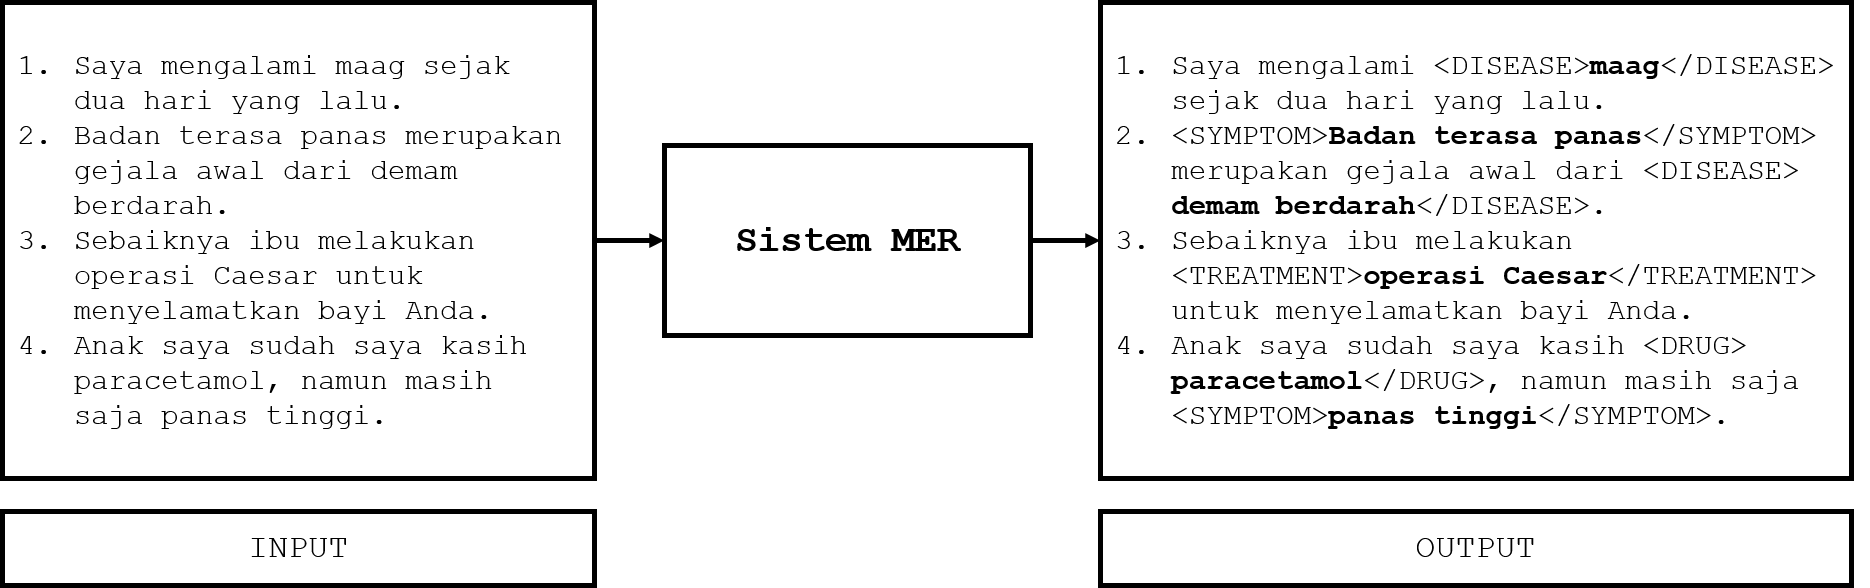
\includegraphics[width=1.0\linewidth]{images/mer_ilustration}
	\caption{Ilustrasi Sistem \mer}
	\label{fig:mer_ilustration}
\end{figure}

Dari ilustrasi di atas, sebuah sistem MER akan diberikan \textit{input} berupa dokumen kesehatan, kemudian sistem diharapkan dapat memberikan \textit{output} berupa dokumen yang sudah diberi label dengan benar. Dokumen kesehatan yang menjadi \textit{input} dapat berupa dokumen formal seperti dokumen suatu rumah sakit atau dokumen non-formal seperti dokumen forum kesehatan \textit{online}.

% Manfaat MER %
Implementasi sistem \mer~dapat memberikan manfaat pada beberapa bidang, seperti pada aplikasi \textit{Question Answering} \citep{abacha2011medical} yang hasil pelabelan dari sistem \mer~dapat mempermudah identifikasi entitas yang ditanyakan. Selain itu, hasil pelabelan sistem \mer~juga dapat dimanfaatkan untuk pembuatan sistem \textit{indexing} dokumen forum sehingga pencarian dokumen kesehatan dapat dilakukan dengan lebih efisien. Sistem \mer~juga dapat digunakan untuk mendukung aplikasi \textit{entity linking} yang memungkinkan seseorang untuk mengetahui hubungan antar entitas \citep{hachey2013evaluating}. Misalnya dengan adanya aplikasi \textit{entity linking}, kita dapat mengetahui obat apabila hanya diberikan \textit{query} nama penyakit dengan \textit{resource} dokumen-dokumen kesehatan yang telah mendapatkan pelabelan dari sistem \mer. Masih banyak manfaat lain dari implementasi sistem \mer~ini.

% Cerita MER Bahasa Inggris %
Sebelumnya \cite{abacha2011medical} telah melakukan penelitian terkait sistem \mer~pada dokumen berbahasa Inggris. Sistem \mer~yang dibuat bertujuan untuk melabeli entitas \textit{treatment}, \textit{problem} dan \textit{test} dengan menggunakan 3 metode, yaitu (i) metode semantik dengan menggunakan \textit{tools} MetaMap (\textit{domain knowledge}), (ii) ekstraksi frasa berdasarkan \textit{chunker} dan klasifikasi dengan SVM (\textit{Support Vector Machine}) dan (iii) gabungan 2 metode sebelumnya dengan menggunakan CRF (\textit{hybrid}). Metode \textit{hybrid} yang dimaksud yaitu dengan menggunakan \textit{tools} CRF sebagai \textit{tools machine learning} yang ditambahkan fitur \textit{domain knowledge}, yaitu fitur semantik yang diekstraksi dengan \textit{tools} MetaMap. Hasil yang terbaik didapatkan dengan menggunakan metode \textit{hybrid} yang menggabungkan 2 metode sebelumnya (\textit{domain knowledge} dan \textit{machine learning}) dan dengan \textit{precision} $ 72.18\% $, \textit{recall} $ 83.78\% $ dan \textit{f-measures} $ 77.55\% $.

Selain penelitian di atas, \cite{mujiono2016new} juga melakukan penelitian terkait \mer~pada dokumen berbahasa Indonesia. Model \mer~yang dikembangkan adalah untuk melabeli entitas \textit{drug} saja. Penelitian tersebut bertujuan untuk mendapatkan representasi data yang berdasarkan karakteristik \textit{training data}. \cite{mujiono2016new} mengusulkan tiga teknik representasi data yang berdasarkan karakteristik distribusi kata dan kemiripan kata dari hasil \textit{training} dari model \textit{word embedding}. Representasi data yang dimasud adalah: (i) semua kalimat diformat sebagai \textit{sequence} token, (ii) semua kalimat di-\textit{generate} menjadi beberapa \textit{sequence}, dan (iii) data direpresentasikan sebagai vektor dengan \textit{tools} \textit{Word Embedding}. Masing-masing representasi kata tersebut dievaluasi dengan masing-masing evaluator, yaitu (i) evaluasi dengan model \textit{neural networks} standar, (ii) evaluasi dengan dua \textit{deep network classifiers}, yaitu DBN (\textit{Deep Belief Networks}), dan SAE (\textit{Stacked Denoising Encoders}) serta (iii) representasi kalimat sebagai vektor \textit{word embedding} yang dievaluasi dengan \textit{recurrent neural networks} yaitu LSTM (\textit{Long Short Term Memory}). Hasil yang didapatkan yaitu kalimat sebagai \textit{sequence} yang dievaluasi dengan LSTM memberikan hasil yang terbaik, yaitu \textit{f-measure} $ 86.45\% $.

% Cerita MER Bahasa Indonesia (Kak Radit, Performa, Tabel) %
Penelitian terkait \mer~pada dokumen berbahasa Indonesia sudah dilakukan sebelumnya oleh \cite{skripsiKakRadit}. Dalam penelitiannya, \cite{skripsiKakRadit} menggunakan CRF (\textit{Conditional Random Fields}) untuk proses pelabelan. Kemudian, pada pekerjaan yang Herwando (2006) lakukan, sebagian besar digunakan untuk mencari fitur-fitur yang memang diskriminatif untuk masalah \mer~yang menghasilkan akurasi terbaik. Entitas yang akan diberi label yaitu nama penyakit (\textit{\disease}), gejala penyakit (\textit{sympton}), obat (\textit{\drug}) dan langkah penyembuhan \textit{\treatment}. Dokumen yang menjadi \textit{input} penelitian merupakan hasil \textit{crawling} dari  forum kesehatan \textit{online} dari berbagai situs yang berisi tanya jawab. Hasil yang didapatkan yaitu \textit{precision} $ 70.97\% $, \textit{recall} $ 57.83\% $ dan \textit{f-measeure} $ 63.69\% $ dengan fitur \textit{its own word}, frasa, kamus (\textit{symptom}, \textit{disease}, \textit{treatment} dan \textit{drug}), \textit{window feature (previous word)} dan panjang kata.

Selain itu, \cite{suwarningsih2014imner} juga melakukan penelitian terkait \mer~pada dokumen berbahasa Indonesia dengan menggunakan SVM (\textit{Support Vector Machine}), dengan SVM yang digunakan untuk klasifikasi per-kata. Entitas yang akan dikenali yaitu \textit{location}, \textit{facility}, \textit{diagnosis}, \textit{definition} dan \textit{person}. Data yang digunakan sebagai korpus merupakan data dari situs \textit{http://health.detik.com/}, \textit{http://detikhealth.com/} dan \textit{http://health.kompas.com/konsultasi/} dengan total keseluruhan sebanyak 1000 kalimat. Akurasi yang dihasilkan yaitu $ 90\% $ dengan menggunakan fitur \textit{baseline}, \textit{word level (morphology, POS-Tag, dll)} dan fitur dari dalam dokumen tersebut.

\section{Deep Learning}
\textit{Deep Learning}, atau disebut juga \textit{deep structured learning, hierarchical learning,} dan \textit{deep machine learning} merupakan salah satu cabang dalam \textit{machine learning} yang model komputasinya terdiri dari beberapa layer mampu mempelajari dan mengekstrak representasi data/fitur secara otomatis pada abtraksi tingkat tinggi \citep{lecun2015deep}. Model tersebut memberikan hasil yang sangat baik dalam penelitan di berbagai bidang seperti \textit{speech recognition}, \textit{object detection}, \textit{sequence labeling} dan lain sebagainya.  

Struktur pembelajaran pada \textit{deep learning} berbentuk hierarki karena termotivasi dari bagaimana neokorteks pada otak maunusia bekerja secara mendalam. Neokorteks tersebut melakukan proses pemelajaran berlayer dan secara otomatis mampu mengketrak fitur dan melakukan abstraksi dari \textit{resource} yang diberikan \citep{bengio2007scaling}. Struktur tersebut terdiri atas \textit{input layer}, \textit{hidden layer} dan \textit{output layer}. \textit{Input layer} memiliki fungsi sebagai tempat masuknya data yang akan dipelajari oleh model. \textit{Hidden layer} melakukan aproksimasi fungsi untuk mendapatkan target dari data \textit{training} yang diberikan. Disebut \textit{hidden layer} karena pada layer ini, \textit{output} tidak bisa kita lihat \citep{Goodfellow-et-al-2016-Book}. \textit{Hidden layer} inilah yang menjadi \textit{key role} dalam \textit{deep learning}. Sedangkan \textit{output layer} merupakan layer untuk mengembalikan target yang diinginkan.

\textit{Deep learning} ini mampu memberikan model yanng memiliki performa sangat baik dalam \textit{supervised learning} \citep{Goodfellow-et-al-2016-Book}. Dengan menambahkan lebih banyak layer dan unit di dalam layer, \textit{deep network} dapat merepresentasikan fungsi dengan kompleksitas yang tinggi. Secara umum, \textit{deep learning} memetakan \textit{input vector} ke \textit{output vector}. Walaupun hal ini mudah dilakukan oleh manusia secar manual, namun untuk \textit{dataset} yang sangat besar, tentu hal ini tidak mungkin dilakukan. Ada banyak macam model \textit{Deep Learning} yang sesuai dengan kebutuhan komputasi, seperti \textit{Deep Belief Network} \citep{hinton2006fast}, \textit{Recurrent Neural Networks} \citep{elman1990finding}, \textit{Long Short Term Memory} \citep{hochreiter1997long}, \textit{Restricted Boltzman Machine} \citep{pennington2014glove} dan lain sebagainya. 

\section{Recurrent Neural Networks}\label{sec:rnns}

\textit{Recurrent neural networks} (RNNs) merupakan merupakan salah satu arsitektur \textit{Deep Learning} yang memiliki koneksi siklik \citep{graves2012neural}. RNNs memiliki \textit{neuron} yang terkoneksi dengan \textit{neuron} lain sehingga membentuk \textit{loop} umpan balik (\cite{haykin2009neural}), tidak seperti \textit{feedforward neural network} (FNNs) dimana aliran informasi hanya berjalan searah. RNNs memungkinkan \iob~yang dihasilkan akan menjadi \ioa~untuk menghasilkan \iob~yang lain. Hal ini menyebabkan perilaku RNNs tidak hanya bergantung pada \ioa~saat ini saja, namun juga bergantung pada \iob~sebelumya. Oleh karena itu, RNNs memiliki kemampuan yang sangat bagus sebagai model dalam permasalahan \textit{sequence data} dibandingkan dengan FNNs. RNNs sendiri memiliki kemampuan yang sangat bagus dalam beberapa \textit{task}, seperti \textit{language model} (\cite{mikolov2010recurrent}) dan \textit{speech recognition} (\cite{graves2013speech}).

Dibandingkan dengan FNNs, RNNs memiliki beberapa kelebihan \citep{mikolov2010recurrent}, yaitu:
\begin{enumerate}
	\item Pada RNNs, kata-kata sebelumnya direpresentasikan dengan \textit{recurrent connections}, sehingga RNNs dapat menyimpan informasi kata sebelumnya dalam jumlah tak hingga. FNNs tidak bisa secara alami memodelkan hubungan kontekstual antara sebuah kata dengan kata-kata pada posisi sebelumnya dan representasi kata sebelumnya berupa konteks dari $ n-1 $ kata. Oleh karena itu, FNNs terbatas dalam penyimpanan informasi kata sebelumnya terbatas seperti pada model \textit{n-gram}.
	\item RNNs dapat melakukan kompresi keseluruhan riwayat kata menjadi ruang dimensi yang lebih kecil, sedangkan FNNs melakukan kompresi/proyeksi hanya dengan sebuah kata saja.
\end{enumerate}

Banyak variasi RNNs yang telah diusulkan oleh beberapa peneliti, seperti Elman \textit{networks} \citep{elman1990finding}, Jordan \textit{networks} \citep{jordan1986attractor}, \textit{time delay neural networks} \citep{lang1990time} dll. Gambar berikut merupakan conroh  dari RNNs secara umum

\begin{figure}
	\centering
	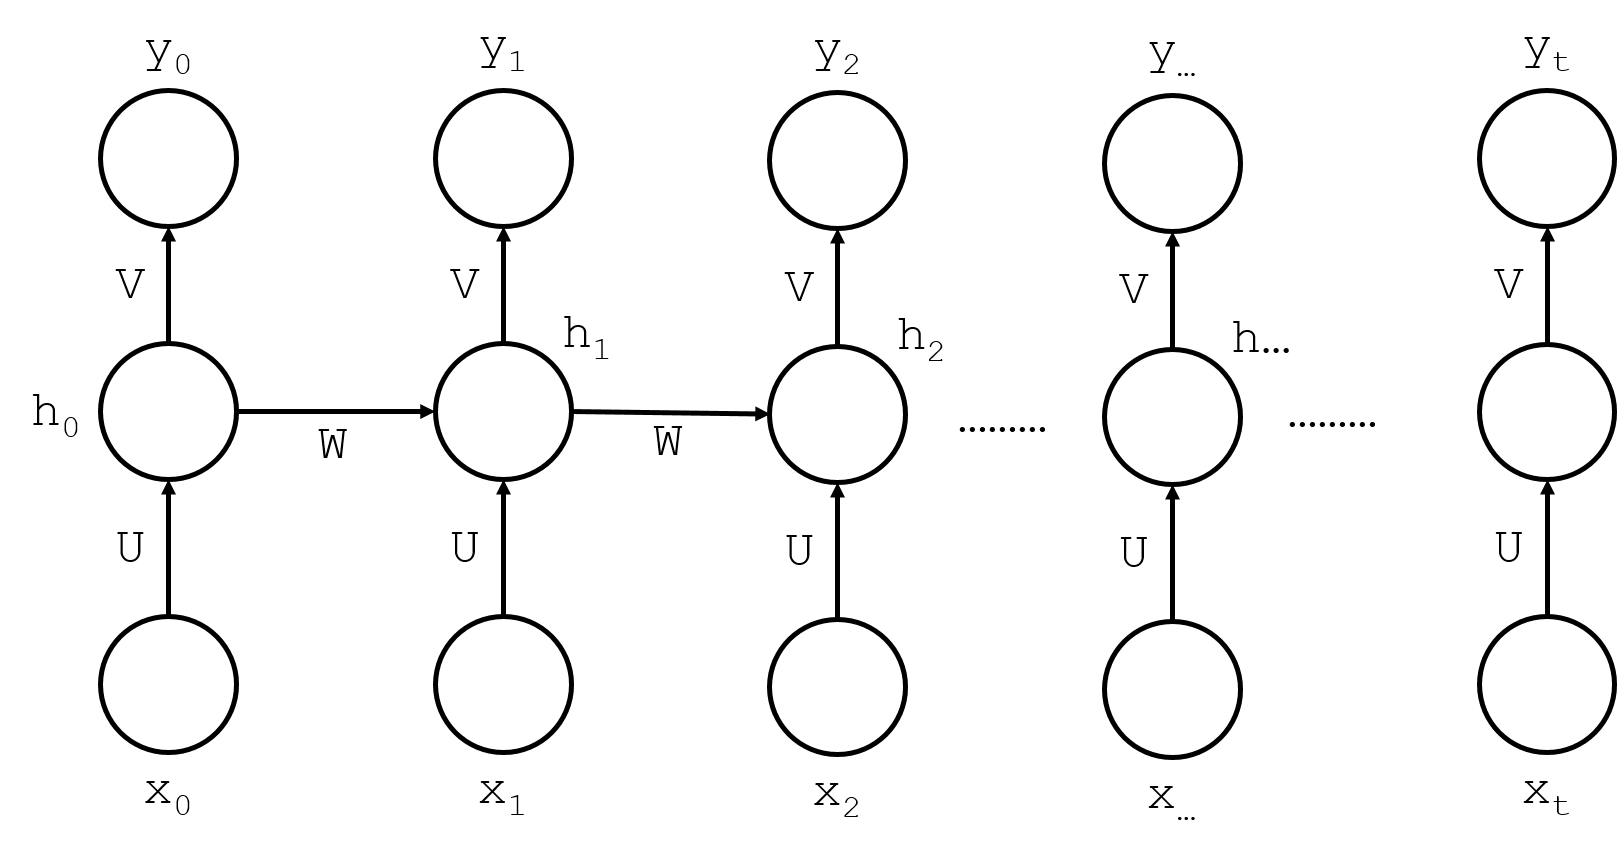
\includegraphics[width=0.80\linewidth]{images/simple_rnn}
	\caption{\textit{Recurrent Neural Networks} sederhana}
	\label{fig:simple_rnn}
\end{figure}

Dari gambar \ref{fig:simple_rnn}, sebuah jaringan pada RNNs memiliki 3 layer pada setiap \textit{timestep}, yaitu \textit{input layer}, \textit{hidden layer} dan \textit{output layer}. \textit{Input layer} merupakan layer sebagai tempat masuk \textit{resource}. Di dalam \textit{hidden layer} tersebut terdapat beberapa unit untuk menyimpan informasi dari \textit{timestep} sebelumnya. Sedangkan pada \textit{output layer} merupakan layer yang memberikan \textit{output} dari model. Pada setiap \textit{timestep} $ t $, RNNs di atas memiliki sebuah \textit{input layer} $ \vec{x(t)} \in {\rm I\!R^{N}} $, \textit{hidden layer} $ \vec{h(t)} \in {\rm I\!R^{H}} $, dan \textit{output layer} $ \vec{y(t)} \in {\rm I\!R^{M}} $. Nilai $ N $, $ H $, dan $ M $ merupakan panjang vektor \textit{input}, jumlah unit di dalam \textit{hidden layer} tersebut, dan panjang vektor \textit{output} yang diinginkan. Terdapat tiga parameter yang akan diestimasi, yaitu $ U \in {\rm I\!R^{H \times N }} $, $ V \in {\rm I\!R^{M \times H}}$, dan $ W \in {\rm I\!R^{H \times H}}$. Tiga parameter tersebut bersifat \textit{shared}, yang artinya masing-masing \textit{timestep} menggunakaan dan mengestimasi tiga parameter tersebut.

Apabila tiga parameter di atas sudah diketahui, $ \vec{h(t)} $ dan $ \vec{y(t)} $ dapat dihitung dengan persamaan:
\begin{equation}
\vec{y(t)} = f(V \cdot \vec{(t)})
\end{equation}
\begin{equation}
\vec{h(t)} = f(U \cdot \vec{x(t)} + W \cdot \vec{h(t-1)})
\end{equation}
dimana
\begin{equation}
\vec{h(0)} = f(W \cdot \vec{x(0)})
\end{equation}
dengan $ f $ sebagai \textit{activation function}, misalnya $ tanh $ atau $ softmax $. Untuk lebih jelasnya, berikut merupakan gambar dari satu buah \textit{timestep} di dalam RNNs.
\begin{figure}
	\centering
	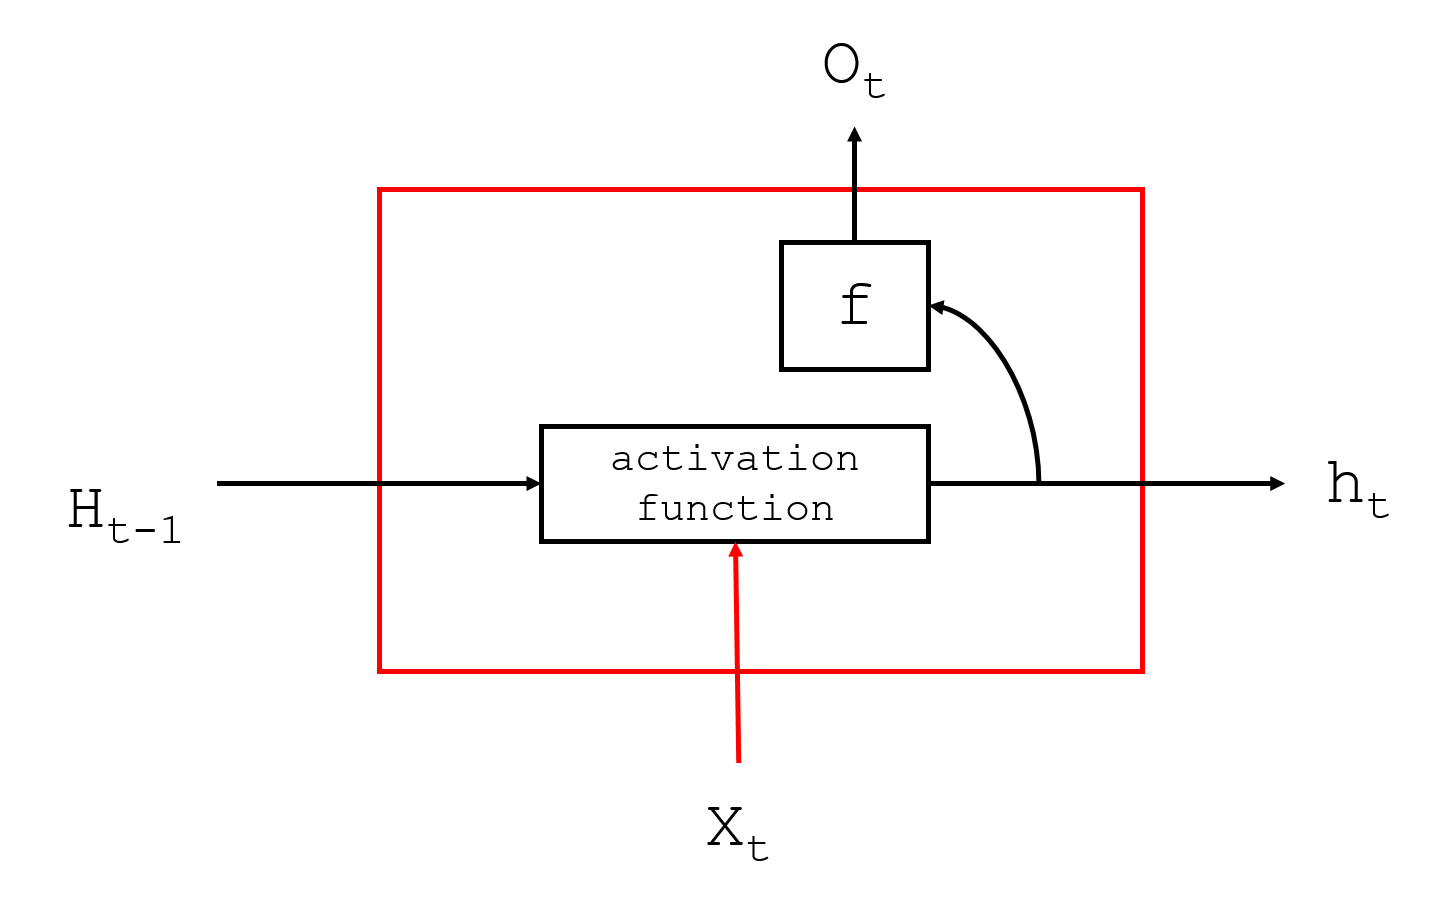
\includegraphics[width=0.80\linewidth]{images/nodes_rnn}
	\caption{1 buah \textit{timestep} dalam RNNs}
	\label{fig:nodes_rnn}
\end{figure}

\subsection{Long Short Term Memory}\label{subbab:lstm}
Pada penjelasan di atas, RNNs memiliki kelebihan mempertimbangkan konteks untuk mengolah \textit{input} menjadi \textit{output}. Sayangnya, \textit{range} konteks yang dapat digunakan dalam satu blok terbatas \citep{graves2012neural}. Efek dari keterbatasan ini yaitu informasi pada suatu blok akan hilang atau terganggu dalam perjalanan \textit{timestep} sehingga \textit{output} yang dihasilkan tidak sesuai harapan. Oleh karena itu RNNs tidak dapat menangani permasalahan dependensi jangka panjang. Permasalahan ini disebut dengan \textit{vanishing gradient problem} (\cite{hochreiter1991untersuchungen}; \cite{hochreiter2001gradient}; \cite{bengio1994learning}). Banyak upaya untuk mengatasi masalah ini, seperti dengan menggunakan \textit{simulated annealing} dan \textit{discrete error propagation} \citep{bengio1994learning}, menggunakan \textit{time delays} (\cite{lang1990time}; \cite{bakker2001reinforcement}) atau \textit{time constant} \citep{ieee1997advances}, dan \textit{hierarchical sequence compression} \citep{schmidhuber2007training}. Namun sejauh ini solusi yang paling bagus yaitu dengan arsitektur \textit{Long Short Term Memory} (LSTM) \citep{hochreiter1997long}.

\begin{figure}
	\centering
	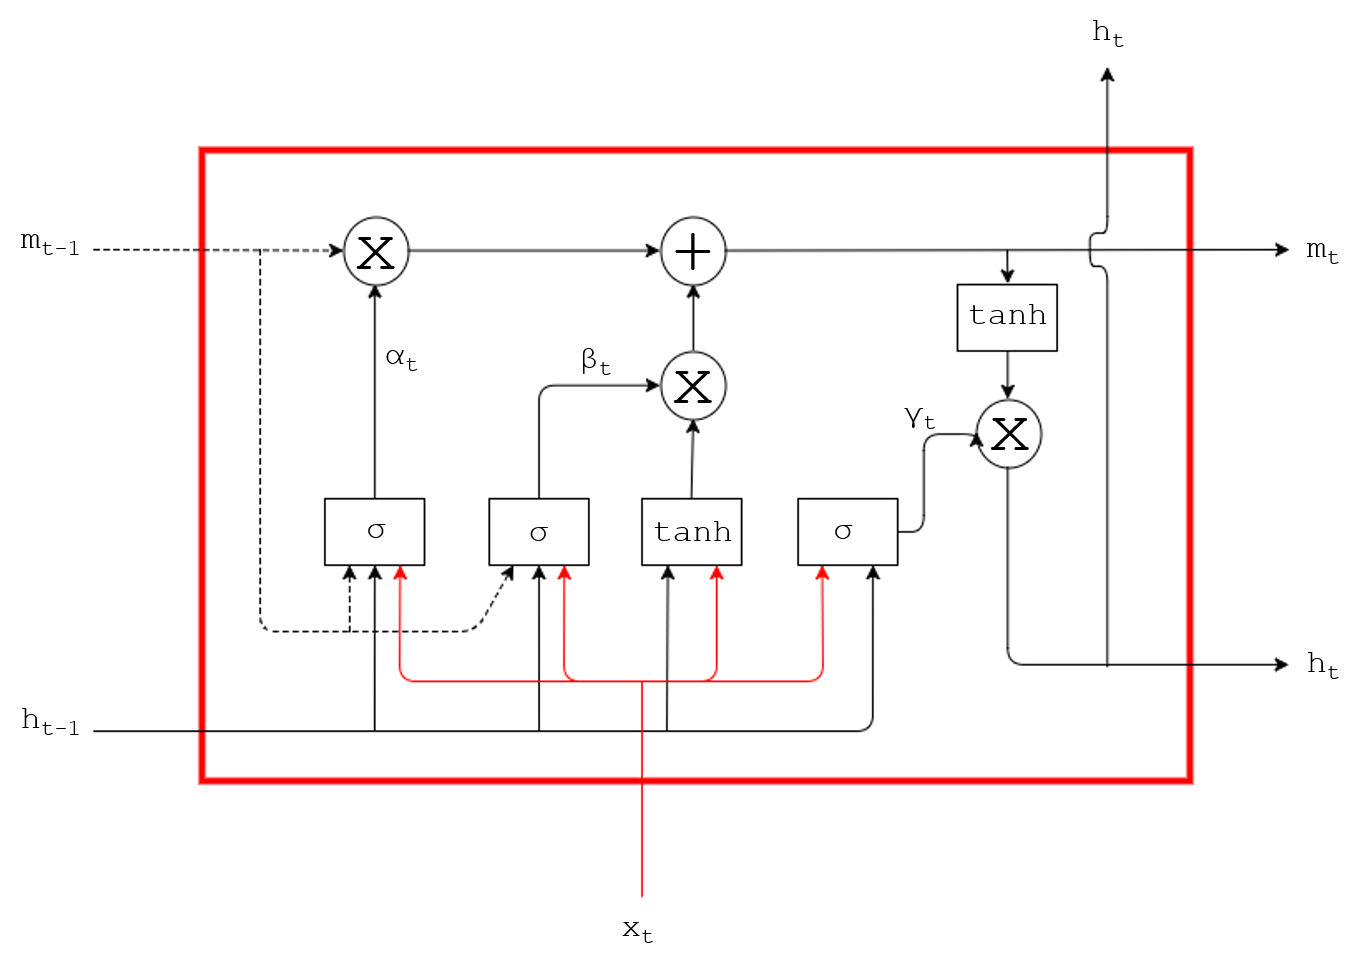
\includegraphics[width=1.0\linewidth]{images/lstm}
	\caption{1 buah blok memori dalam LSTM}
	\label{fig:lstm}
\end{figure}

LSTM diperkenalkan oleh \cite{hochreiter1997long} dan saat ini banyak digunakan dalam berbagai \textit{task}. Gambar \ref{fig:lstm} merupakan ilustrasi satu buah blok memori di dalam LSTM. Pada dasarnya, arsitektur LSTM mirip dengan RNNs, namun unit \textit{nonlinear} pada \textit{hidden layer} di dalam RNNs diganti menjadi blok memori. Sebuah blok memori memiliki gerbang \textit{multiplicative} yang berfungsi untuk menyimpan dan mengakses informasi dari blok sebelumnya namun dengan batasan yang jauh lebih besar dibanding RNNs, sehingga mampu menghindari \textit{vanishing gradient problem}. Apabila \textit{input gate} selalu tertutup, maka memori tidak akan perah ditimpa sehingga isi memori tidak berubah.

Pada gambar \ref{fig:lstm}, kita dapat melihat bahwa 1 blok memori pada LSTM tersebut memiliki 3 buah gerbang, yang berfungsi untuk sebagai pengatur suatu informasi apakah ditambahkan, dipertahankan atau dihapus di dalam sebuah sel. Masing-masing gerbang terdiri dari komponen \textit{sigmoid layer} dan komponen untuk melakukan operasi penjumlahan atau perkalian untuk masing-masing \textit{element-wise}. \textit{Sigmoid layer} tersebut memiliki nilai antara nol sampai dengan satu, yang mendeskripsikan perilaku gerbang dalam menerima \textit{input}. Semakin kecil nilai dari layer tersebut maka semakin kecil pula informasi masuk ke gerbang terkait dan sebaliknya. 

\begin{enumerate}
	\item \textit{Forget Gate}\\
	Gerbang ini memiliki fungsi untuk menentukan informasi yang akan disimpan di dalam memori dengan formula berikut
	\begin{equation}\label{eq:forget_lstm}
	\alpha_{t}=\sigma(W_{x\alpha}+W_{h\alpha}\cdot~h_{t-1}+W_{m\alpha}\cdot~m_{t-1})
	\end{equation}
	
	\item \textit{Input Gate}\\
	Gerbang ini berfungsi untuk menentukan apakah informasi baru $ x(t) $ akan disimpan dalam \textit{cell state} atau tidak. 
	\begin{equation}\label{eq:input_lstm}
	\beta_{t}=\sigma(W_{x\beta}+W_{h\beta}\cdot~h_{t-1}+W_{m\beta}\cdot~m_{t-1})
	\end{equation}
	
	\item \textit{Output Gate}\\
	Gerbang ini berfungsi untuk menendukan \textit{output} dari sebuah \textit{timestep} berdasarkan \textit{cell state} saat ini.
	\begin{equation}\label{eq:output_lstm}
	\gamma_{t}=\sigma(W_{x\gamma}+W_{h\gamma}\cdot~h_{t-1}+W_{m\gamma}\cdot~m_{t-1})
	\end{equation}
	
\end{enumerate}

Dalam setiap \textit{timestep} $ t $, berikut merupakan formula untuk menghitung $ m(t) $ dan $ h(t) $:
\begin{equation}\label{eq:mt}
m_{t}=\alpha_{t} (\times) m_{t-1} + \beta_{t} (\times) f(x_{t},{t-1})
\end{equation}
\begin{equation}\label{eq:ht}
h_{t}=\gamma_{t} (\times) tanh(m_{t})
\end{equation}
dimana
\begin{equation}\label{eq:hf}
f(x_{t},{t-1})=tanh(W_{xm} \cdot x_{t} + W_{hm} \cdot h_{t-1})
\end{equation}

Notasi $ (\times) $ merupakan operasi perkalian untuk setiap pasang elemen, dan $ (+) $ merupakan operasi penjumlahan setiap pasang elemen.

\subsection{Penerapan RNNs untuk MER}
Terdapat beberapa penelitian terkait \mer~yang dikembangkan menggunakan RNNs, seperti \textit{drug entity recognition} \citep{mujiono2016new}, \textit{medical event detection on EHR} \citep{jagannatha2016bidirectional}, \textit{biomedical entity recognition} \citep{limsopatham2016learning}, dan \textit{Named Entity Recognition in Swedish Health Records} \citep{almgren2016named}. Penelitian \textit{drug entity recognition} oleh \cite{mujiono2016new} sudah dijelaskan pada subbab \ref{aboutmer}.

Dalam penelitiannya, \cite{jagannatha2016bidirectional} menggunakan LSTMs untuk memprediksi label entitasnya. Penelitian tersebut bertujuan untuk mendeteksi kejadian medis pada \textit{Electronic Health Records} seperti \textit{ medication, diagnosis (Indication), adverse drug events (ADEs) severity, other SSD, frequency, drugname} dan \textit{duration}. Sebagai pembanding, penulis tersebut juga mengimplementasikan CRF dan GRU. Ada beberapa kesulitan yang dihadapi dalam mengolah EHR tersebut, yaitu EHR lebih \textit{noisy} dibandingkan dengan teks biasa, banyak kalimat yang tidak komplet dan penggunaan frasa. Hasil dari penelitian tersebut menunjukkan bahwa semua model RNNs (LSTMs dan GRU) memiliki akurasi yang lebih baik daripada CRF. Apabila dibandingkan dengan \textit{baseline} yang digunakan, GRU mampu meningkatkan \textit{recall} (0.8126), \textit{precision} (0.7938) dan \textit{F-score} (0.8031) sebesar 19\%, 2\% dan 11\%.

\cite{limsopatham2016learning} menggunakan \textit{Bidirectional-LSTMs} untuk mengidentifikasi kalimat dengan menggunakan karakter dan kata yang diubah menjadi vektor menggunakan \textit{word embedding}. Untuk setiap kalimatnya, peneliti tersebut mengusulkan adanya \textit{ortographic feature} supaya modelnya dapat mempelajari fitur tersebut secara eksplisit. Evaluasi yang digunakan menggunakan tiga buah koleksi \textit{biomedical test}, yaitu \textit{Gene Mention task corpus}, \textit{BioNLP 2009} dan \textit{NCBI disease corpus}, dengan perhitungan \textit{F1-score}. ada empat \textit{baseline} yang digunakan sebagai pembanding, yaitu \textit{feedforward}, \textit{bidirectional-LSTM}, \textit{CNN-Bidirectional-LSTM} yang hanya menggunakan karakter dan \textit{CNN-Bidirectional LSTM}. Hasil yang didapatkan mengatakan bahwa penggunaan \textit{Bidirectional-LSTM} yang dikombinasikan dengan CNN dengan diberikan \textit{word embedding} dan \textit{orthographic} merupakan model yang paling bagus. Penulis tersebut juga menyimpulkan bahwa penggunaan fitur \textit{hand-crafted} tersebut mampu memberikan akurasi yang lebih tinggi.

\cite{almgren2016named} menggunakan \textit{deep bidirectional LSTM} dalam mengembangkan NER di bidang medis. Entitas yang akan diidentifikasi adalah \textit{disorders and findings}, \textit{pharmaceutical drugs}, \textit{body structure} dan \textit{non-entity term}. Model menggunakan teks medis berbahasa Swedia sebagai \textit{dataset}, di-\textit{train} dengan menggunakan \textit{end-to-end backpropagation} dan Adam \textit{optimizer}, dan \textit{input} yang diberikan berbentuk urutan karakter. \textit{Baseline} yang digunakan yaitu \textit{Stockholm EPR corpus}, yang mana mendapatkan \textit{precision} 0.67, \textit{recall} 0.12 dan \textit{f-measure} 0.20. Hasil yang didapatkan adalah Char-BiLSTM pada Stockholm EPR corpus memiliki \textit{precision} tyang lebih tinggi (0.67), dan \textit{recall} yang juga lebih tinggi (0.24) dibandingkan dengan \textit{baseline}.

\section{Word Embedding}
Pada umunya, pendekatan yang digunakan untuk merepresentasikan sebuah kata sebagai \textit{input} model adalah dengan menggunakan \textit{one-hot-vetor} \citep{turian2010word}. Panjang dari sebuah vektor kata ini bergantung dari banyaknya kata unik di dalam sebuah korpus. Ada beberapa cara untuk mengubahnya menjadi \textit{one-hot-vector}, seperti mengumpulkan semua kata unik kemudian mngurutkannya secara alfabetis. Vektor \textit{one-hot} tersebut bernilai 1 pada indeks kata yang bersesuaian. Misalnya kata "obat" berada di indeks ke 25 pada kumpulan kata unik, maka representasi vektornya elemen ke 21 di vektor "obat" adalah 1 sedangkan yang lainnya 0.

Dari ilustrasi singkat tersebut, representasi \textit{one-hot-vector} memiliki kelemahan yaitu besar vektor yang tergantung jumlah kata unik di dalam korpus. Selain itu, jika terdapat sebuah kata yang muncul di korpus namun tidak muncul di \textit{training} ataupun \textit{testing data}, kata tersebut tidak dapat diproses. Selain itu, sangat susah untuk mencari hubungan baik sintaks maupun semantiks dari representasi kata ini, karena antar kata hanya dibedakan indeks yang berisi angka 1 saja.

Dari kelemahan di atas, terdapat sebuah representasi vektor lain dari kata yang lebih baik, yaitu dengan menggunakan \textit{word embedding}. \textit{Word embedding} adalah salah satu jenis dari representasi kata yang memiliki kelebihan yaitu padat, berdimensi rendah, dan memiliki nilai yang real. \textit{Word embedding} memetakan kata dengan vektor berisi bilangan \textit{real}, misalkan W("obat") = [0.4, -0.9, 0.1, ...., 0.9], dimana W adalah fungsi yang memetakan suatu kata menuju representasi vektor dan W("obat") merupakan \textit{word embedding} dari kata "obat". \textit{Word embedding} dapat meningkatkan performa dari \textit{tasks} dalam NLP dengan cara mengelompokkan kata-kata yang mirip, karena kata yang mirip memiliki vektor yang mirip pula. Ada beberapa metode \textit{word embedding} yang banyak digunakan dalam beberapa \textit{task} di NLP, seperti Glove \citep{pennington2014glove} dan Word2Vec \citep{mikolov2014word2vec}. Pada pembahasan ini, \saya~hanya menuliskan mengenai Word2Vec.

Word2Vec merupakan model linguistik yang dikembangkan oleh \cite{mikolov2014word2vec} dan berdasarkan pada \textit{neural networks}. Word2Vec mempelajari \textit{embedding} dari setiap kata untuk dipetakan ke masing-masing vektor yang berdimensi rendah dari sifat distribusinya pada korpus yang diberikan. Dari situ, Word2Vec mampu mengelompokkan kata berdasarkan kemiripannya di dalam \textit{vector space}.

\begin{figure}
	\centering
	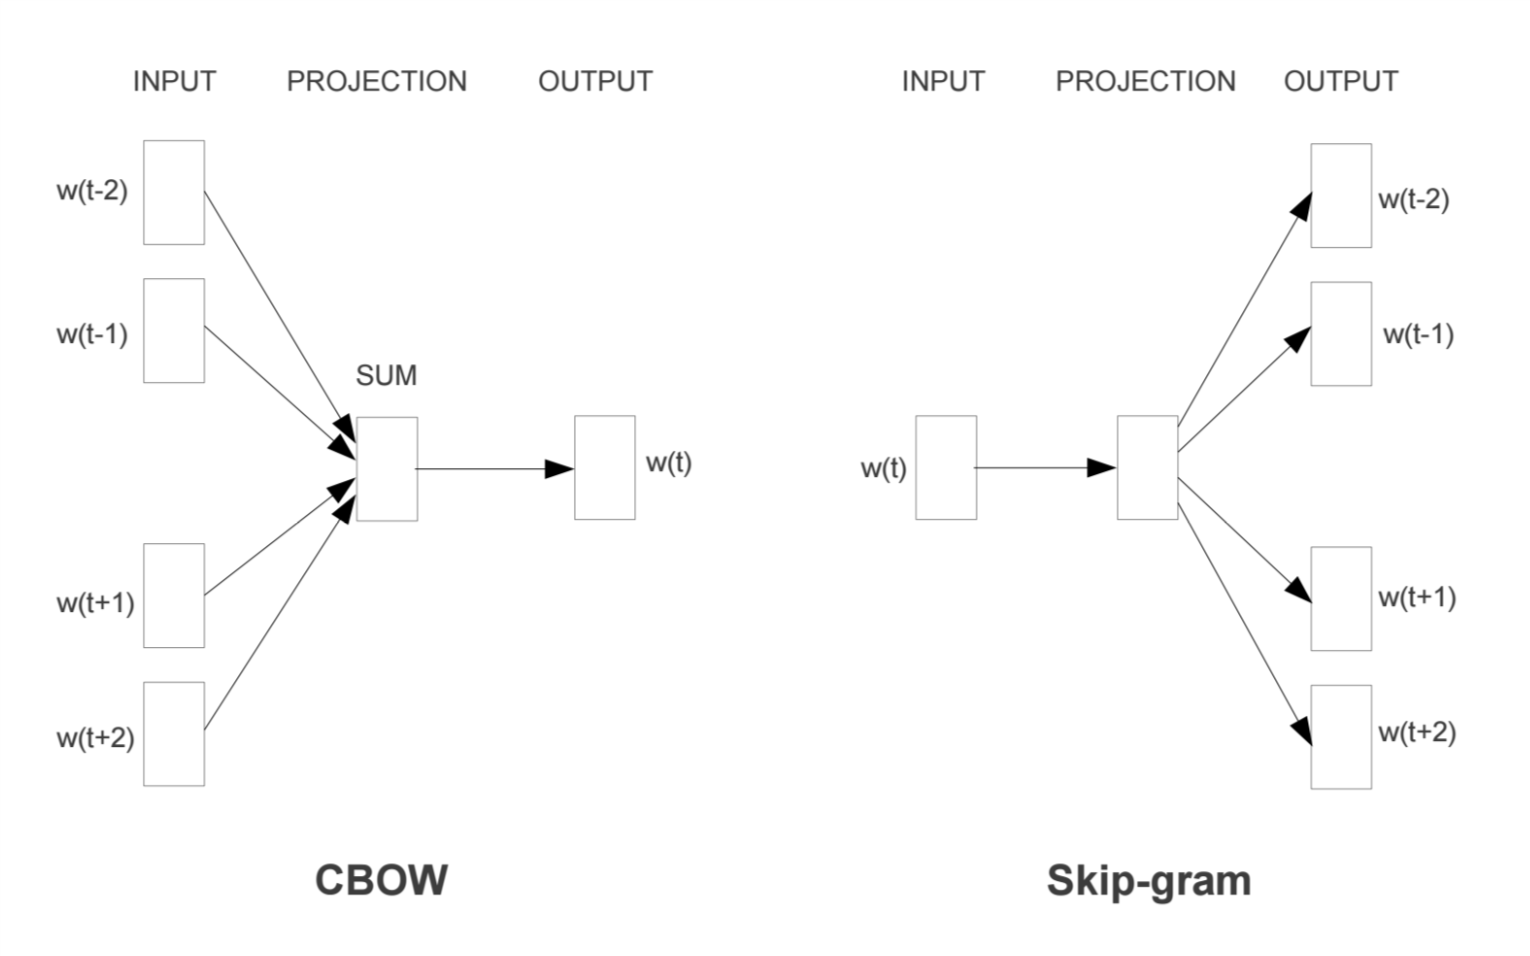
\includegraphics[width=0.85\linewidth]{images/word2vec}
	\caption{Arsitektur Word2Vec}
	\label{fig:word2vec}
\end{figure}

Ada dua arsitektur Word2Vec yang dikembangkan oleh \cite{mikolov2014word2vec}, yaitu arsitektur \textit{skip-gram} dan arsitektur \textit{continuous bag-of-words} (CBOW). Dari gambar \ref{fig:word2vec}, dapat dilihat bahwa arsitektur CBOW memprediksi masing-masing kata berdasarkan kata di sekelilingnya. \textit{Input layer} dalam arsitektur ini direpresentasikan dengan \textit{bag-of-words}. CBOW sendiri dapat mempelajari data dengan ukuran yang sangat besar yang tidak dapat dilakukan oleh model \textit{neural network} yang lain. Sedangkan arsitektur \textit{skip-gram} memprediksi kata-kata di sekeliling dan konteksnya berdasarkan sebuah kata yang diberikan (gambar \ref{fig:word2vec}). \textit{Skip-gram} mampu menangkap \textit{co-occurance} rata-rata dari dua buah kata di dalam \textit{training set}.
%-----------------------------------------------------------------------------%
% Cerita umum Word Embedding terlepas dari, kenapa bukan %
% Salah satunya adalah word2vc%
% CBOW vs Skip %
